\subsection{SOI}
\subsubsection{Collaborating Institutions}
KEK
\subsubsection{Introduction}
\subsubsection{Recent Milestones}
At present, major issues in the SOI pixel development are ``back-gate effect'', ``hole trap under the transistors by radiation,'' and ``sensor-circuit cross talks'' as shown in Figure~\ref{fig:VertexDetector:SOI:SOI_Schematic}. For these, we have been developing a double SOI technology. The developed double SOI wafer has an additional middle-SOI(Si) layer under the transistors. The conduction layer of the middle-SOI can solve all the three issues. We could successfully process the double-SOI wafer (Figure~\ref{fig:VertexDetector:SOI:crossSectionAfterProcessing}). Threshold shift by radiations is successfully recovered by applying compensating voltage to the middle SOI layer (Figure~\ref{fig:VertexDetector:SOI:thresholdShift}).

\begin{figure}
\centering
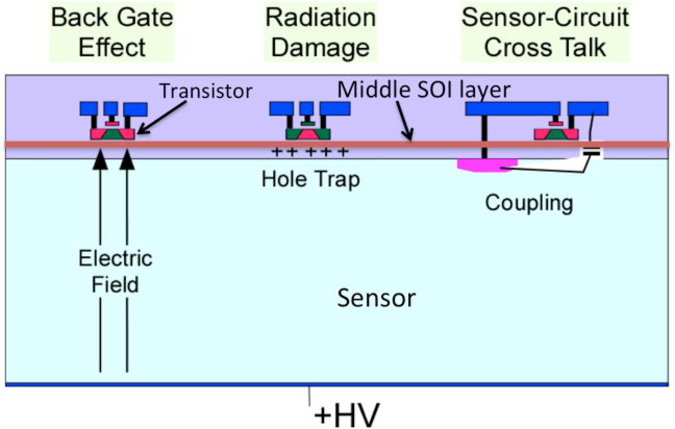
\includegraphics[width=.5\textwidth]{VertexDetector/SOI/SOI_Schematic}
\caption{Major issues in the SOI pixel detector and introduction of a middle-SOI layer}
\label{fig:VertexDetector:SOI:SOI_Schematic}
\end{figure}

\begin{figure}
\centering
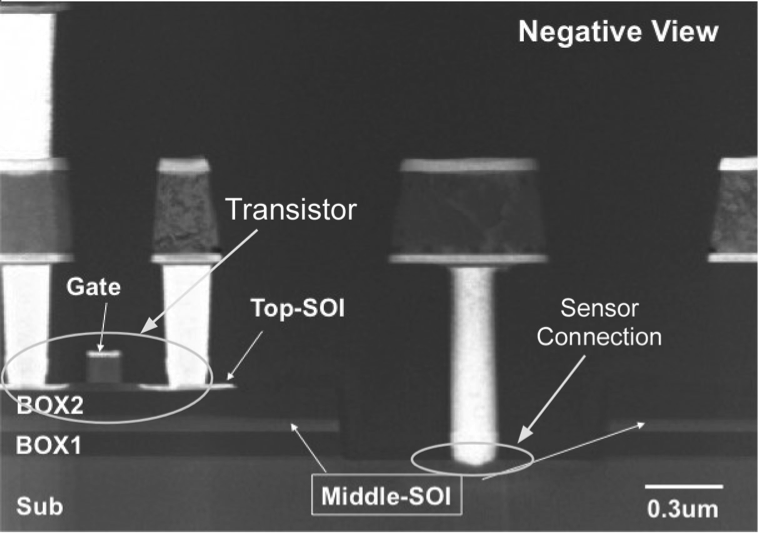
\includegraphics[width=.5\textwidth]{VertexDetector/SOI/crossSectionAfterProcessing}
\caption{Cross section of the double SOI chip after processing}
\label{fig:VertexDetector:SOI:crossSectionAfterProcessing}
\end{figure}

\begin{figure}
\centering
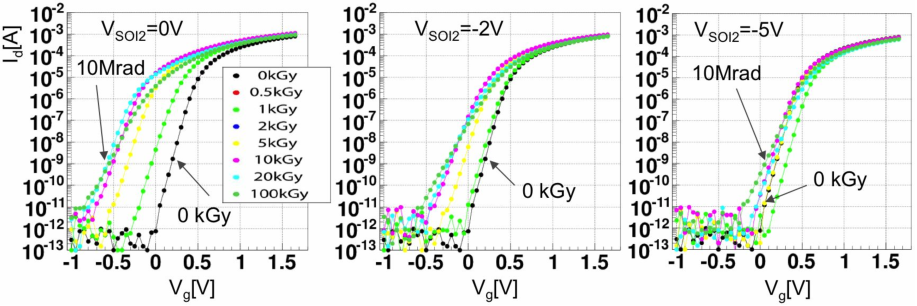
\includegraphics[width=.5\textwidth]{VertexDetector/SOI/thresholdShift}
\caption{Threshold shift recovery by applying compensating voltage (Vsoi2) to the middle Si layer}
\label{fig:VertexDetector:SOI:thresholdShift}
\end{figure}

\subsubsection{Engineering Challenges}
The resolution for the ILC vertex detector is required as better as a few \micron. This means pixel size must be less than \unit[20]{\micron} square or so. On the other hand, each pixel must register arrival time of the hits during bunch train etc., so this requires many transistors and capacitors must be located in each pixel area.
Natural solution to this is 3D vertical integration of circuit layer. SOI technology is very fit to the 3D integration since the thinning is stopped at the buried oxide (BOX). We already tried 3D SOI pixel chip in collaboration with T-Micro Co. Ltd. Process flow of micro-bump 3D connection is shown in Figure~\ref{fig:VertexDetector:SOI:microbump3D}. We have confirmed low resistance (~\unit[6]{$\Omega$}/bump) between upper and lower tiers for 1,000 daisy chain (2,000 bumps) as show in Figure~\ref{fig:VertexDetector:SOI:resistanceOfDaisyChain}.
However, we think much higher density digital circuit such as \unit[32]{nm} technology may be necessary for the upper tier in the ILC. This requires bonding of two different technology wafers. The 3D integration of different technology wafers (or chips) is still engineering challenge.

\begin{figure}
\centering
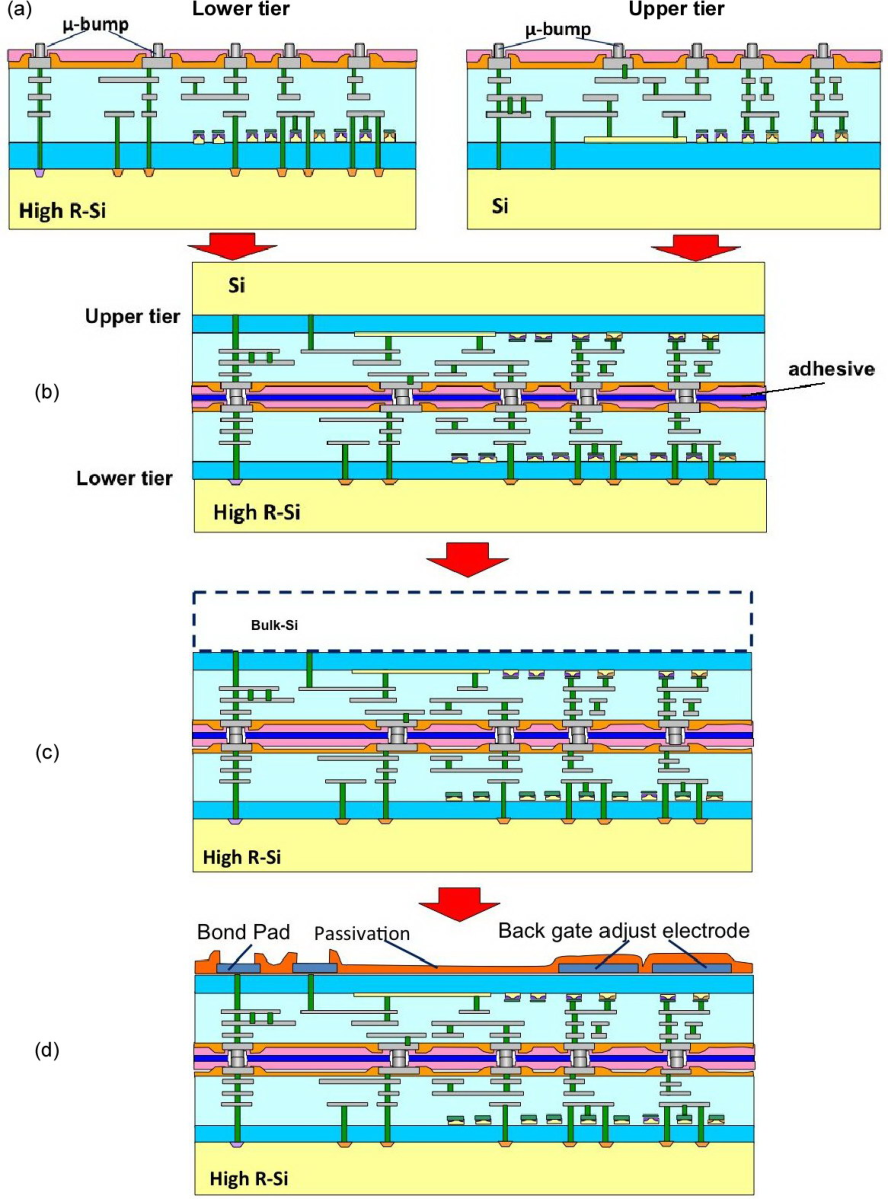
\includegraphics[width=.5\textwidth]{VertexDetector/SOI/microBump3DIntegration}
\caption{Micro-bump 3D integration process flow of the SOI pixel}
\label{fig:VertexDetector:SOI:microbump3D}
\end{figure}

\begin{figure}
\centering
\includegraphics[width=.5\textwidth]{VertexDetector/SOI/resistanceOfDaisyChain}
\caption{Resistance of micro-bump daisy chain between upper and lower tiers}
\label{fig:VertexDetector:SOI:resistanceOfDaisyChain}
\end{figure}

\subsubsection{Future Plans}
Detector R\&D plans for the coming years;
We are planning following items for the coming year.
\begin{itemize}
\item ~Sep. 2014 : Complete architecture study for the ILC pixel detector.
\item ~Mar. 2015 : Design and fabrication of first test chip for the ILC.
\item ~Dec. 2015 : Beam test of the test chip.
\end{itemize}
